\documentclass[t]{beamer}
\usepackage[portuguese]{babel}
\usepackage[utf8]{inputenc}
\usetheme{Berkeley}
\usecolortheme{seahorse}
\usepackage{graphicx}

\addto\captionsportuguese{
	\renewcommand{\figurename}{Fig.}
	\renewcommand{\tablename}{Tab.}
}

\title{Economia Disruptiva}
\subtitle{Como mudar paradigmas em benefício de todos}

\AtBeginSection[]
{
	\begin{frame}
	\frametitle{Sumário}
	\tableofcontents[currentsection]
	\end{frame}
}

\begin{document}

\frame{\titlepage}

\begin{frame}
\frametitle{Sumário}
\tableofcontents
\end{frame}

\section{Disrupção}

\begin{frame}{Definição}
	\begin{itemize}	
		\item Interrupção do curso normal de um processo.
		\item Restabelecimento brusco de corrente elétrica, causando faíscas e intenso gasto da energia acumulada.
		\item É o processo onde uma empresa com poucos recursos pode enfrentar o mercado já estabelecido.  
	\end{itemize}
\end{frame}

\begin{frame}{Exemplos de disrupção}
	\begin{itemize}
		\item Fotolog x Instagram
		\item Taxi x Uber
		\item SMS x Whatsapp
		\item Carta x Email x Videoconferência
		\item Blockbuster x Netflix
	\end{itemize}
\end{frame}

\section{Economia Disruptiva}

\begin{frame}{Economia disruptiva}
	\begin{itemize}
		\item Transição nos setores
		\item Necessidade de reinvenção
		\item Enfrentar novos desafios
		\item Causar impacto
	\end{itemize}
\end{frame}

\begin{frame}{Economia disruptiva}
	\begin{itemize}
		\item Enfrentar novos desafios
		\begin{itemize}
			\item Mercados já estabelecidos
			\begin{itemize}
				\item Tradição
				\item Sócios antigos
			\end{itemize}
			\item Estado
			\begin{itemize}
				\item Leis
				\item Burocracia
			\end{itemize}
			\item Internacionalização
			\begin{itemize}
				\item Cultura
				\item Vandalismo
				\item Lingua/linguagem
			\end{itemize}
		\end{itemize}
	\end{itemize}
\end{frame}

\section{Quadro de Modelo de Negócios}

\begin{frame}{Quadro de Modelo de Negócios}
	\begin{itemize}
		\item Business Model Canvas (BMC)
		\item Ferramenta de gerenciamento estratégico
		\item Permite desenvolver e esboçar modelos de negócio novos
		\item Mapa visual pré-formatado contendo nove blocos do modelo de negócios
	\end{itemize}
\end{frame}

\begin{frame}{Quadro de Modelo de Negócios}
	\begin{figure}
		\centering
		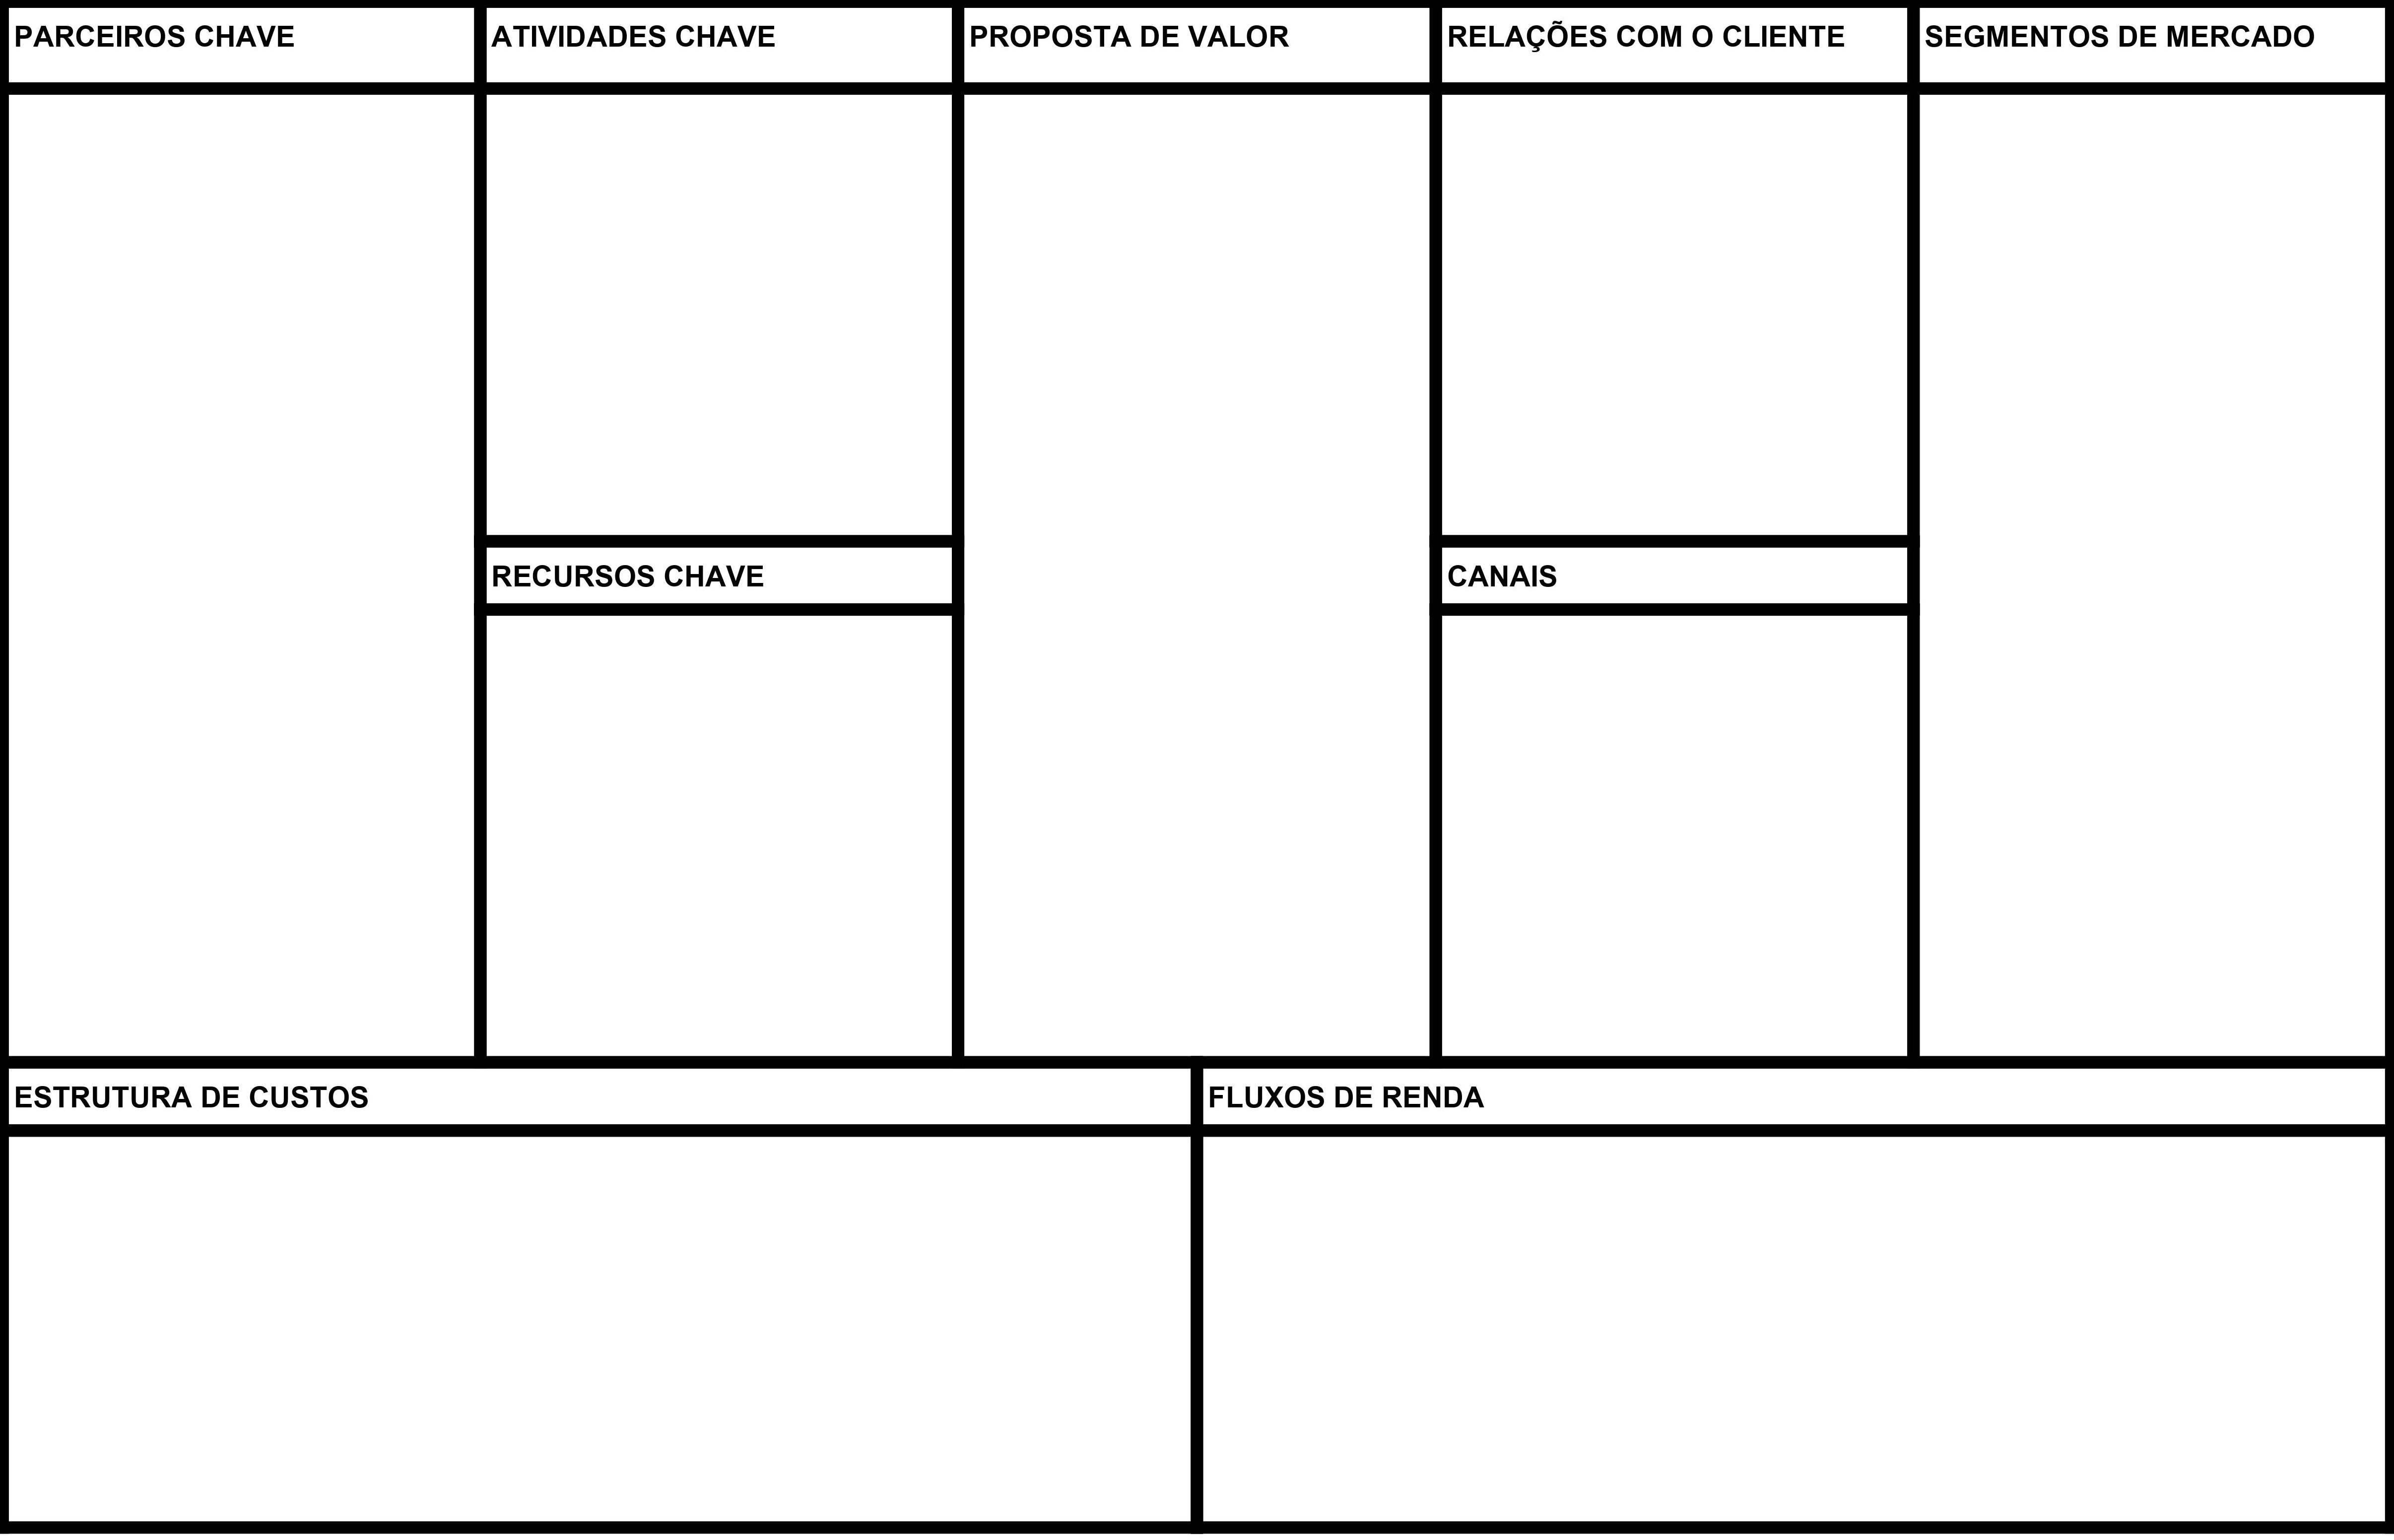
\includegraphics[width=\linewidth]{bmc-pt}
		\caption{Quadro de Modelo de Negócios}
		\label{fig:bmc}
	\end{figure}
\end{frame}

\begin{frame}{Modelo de negócios do 99 táxi}
	\begin{figure}
		\centering
		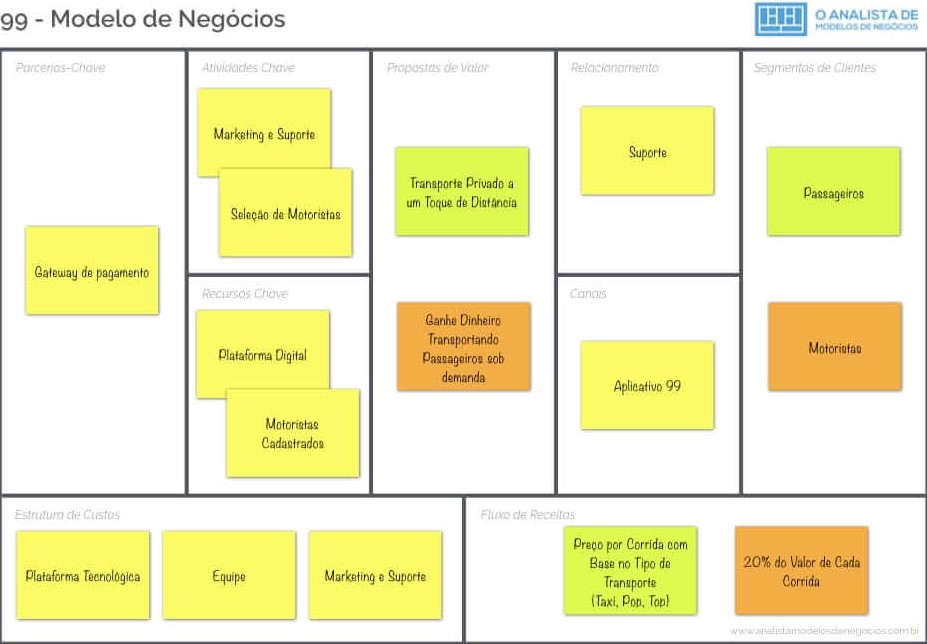
\includegraphics[width=0.9\linewidth]{bmc-99}
		\caption{Modelo de negócios do 99 táxi}
		\label{fig:bmc-99}
	\end{figure}
	
\end{frame}

\section{Observações}

\begin{frame}{Observações}
	\begin{itemize}
		\item Evitar pensar na ideia "promova disrupção, ou ela ocorrerá com você"
		\item Algumas inovações disruptivas podem falhar
		\item Há teorias que definem disrupção inovativa e precisam ser melhor compreendidas:
		\begin{itemize}
			\item De certo ponto de vista, Uber não é uma inovação disruptiva, por exemplo.
		\end{itemize}
	\end{itemize}
\end{frame}

% https://hbr.org/2015/12/what-is-disruptive-innovation
% https://www.slideshare.net/neigrando/what-is-disruptive-innovation-65191386

\frame{\titlepage}

\end{document}
